\documentclass[a4paper,12pt]{article}

\usepackage{geometry}
\usepackage{polski}
\usepackage{amsmath}
\usepackage{ragged2e}
\usepackage{graphicx}
\usepackage{xcolor}
\usepackage{siunitx}
\usepackage{multirow}
\usepackage{pdfpages}

\graphicspath{ {./images/} }

\newcommand\crule[3][black]{\textcolor{#1}{\rule{#2}{#3}}}

\geometry{
 a4paper,
 total={170mm,257mm},
 left=20mm,
 top=20mm,
 }

\definecolor{amethyst}{rgb}{0.6, 0.4, 0.8}

\begin{document}
\title{Układy Elektroniczne - Logika sekwencyjna}
\author{Grzegorz Litarowicz \\ Piotr Moszkowicz} 
\date{\today}
\maketitle
\pagenumbering{roman}

\newpage
\begin{justify}
\tableofcontents
\newpage
\pagenumbering{arabic}

\section{Cel i zakres ćwiczenia}

Celem ćwiczenia było zapoznanie się z logiką sekwencyjną oraz utworzenie prostych układów (liczników).

\section{Wstęp teoretyczny}

\subsection{Logika sekwencyjna}

Logika, w której wyjście zależy nie tylko od wejścia, ale również od stanu poprzedniego, który zwany jest stanem wewnętrznym i jest pamiętany w rejestrze. Dzięki tej właściwości, możemy tworzyć układy, które nie tylko reagują na wejście, ale również zapamiętują swój stan, co jest bardzo powszechnie wykorzystywane - w naszym przypadku przy konstrukcji liczników.

\subsection{Kod Grey'a}
\label{grey}

Kod dwójkowy, który charakteryzuje się tym, iż kolejne wartości (słowa kodowe) różnią się między sobą stanem tylko jednego bitu. Ostatni i pierwszy wyraz tego kodu również spełnia to wymaganie.

\subsection{Przesunięcie bitowe}
\label{przesbit}

Operacja, którą wykonujemy na liczbach binarnych. Polega na zamianie miejscami bitów danej liczby, zależnie w którą stronę wykonujemy przesunięcie. Poniżej pokazany jest przykład przesunięcia bitowego w prawo:

Wejście: 1011
Wyjście: 1101

Jak widać powyżej każdy bit "przeskoczył" w prawo, natomiast ostatni wszedł na miejsce pierwszego.

\section{Schemat płytki PLD}

\begin{figure}[h!]
\centering
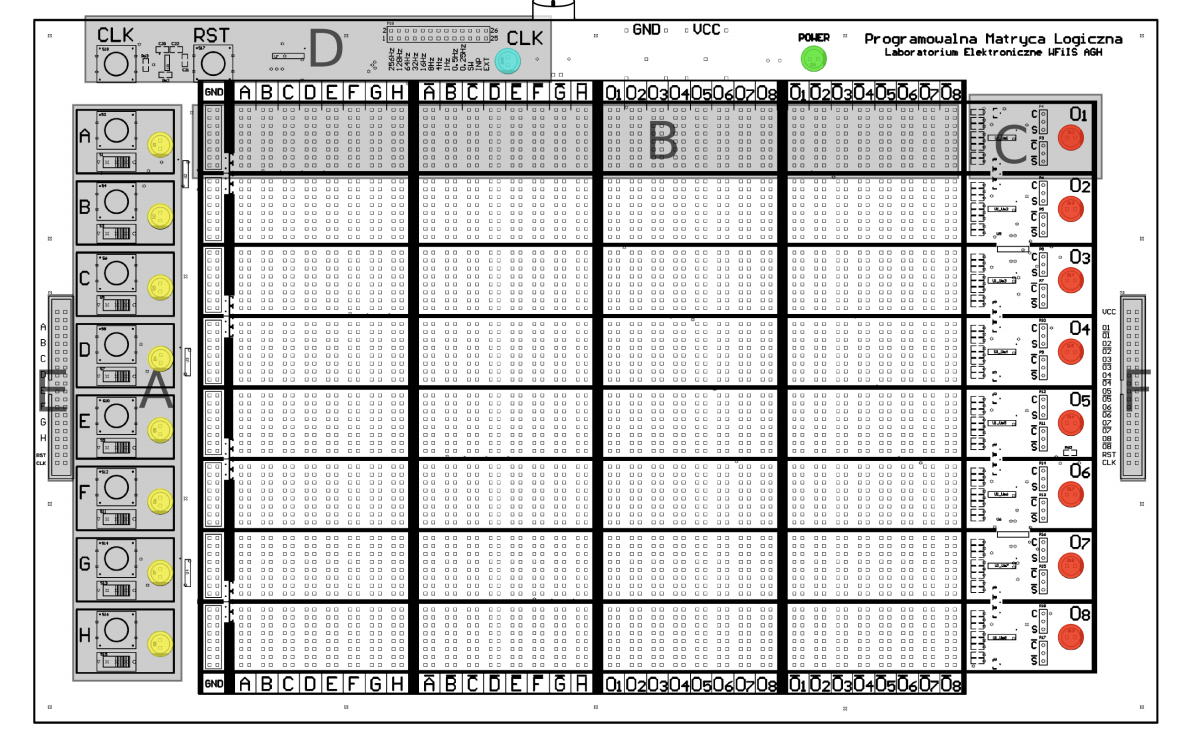
\includegraphics[width=15cm, height=8cm]{pld}
\end{figure}

\section{Pomiary i wyniki}

\subsection{4 bitowy licznik modulo 14}

Jako pierwsze ćwiczenie mieliśmy zaprojektować licznik 4 bitowy, który wykonywał operację modulo 14. Poniżej można zaobserwować zeskanowane tabele Karnaugh'a oraz wzory 4 funkcji, które wykorzystaliśmy do zbudowania tegoż licznika.

\newpage

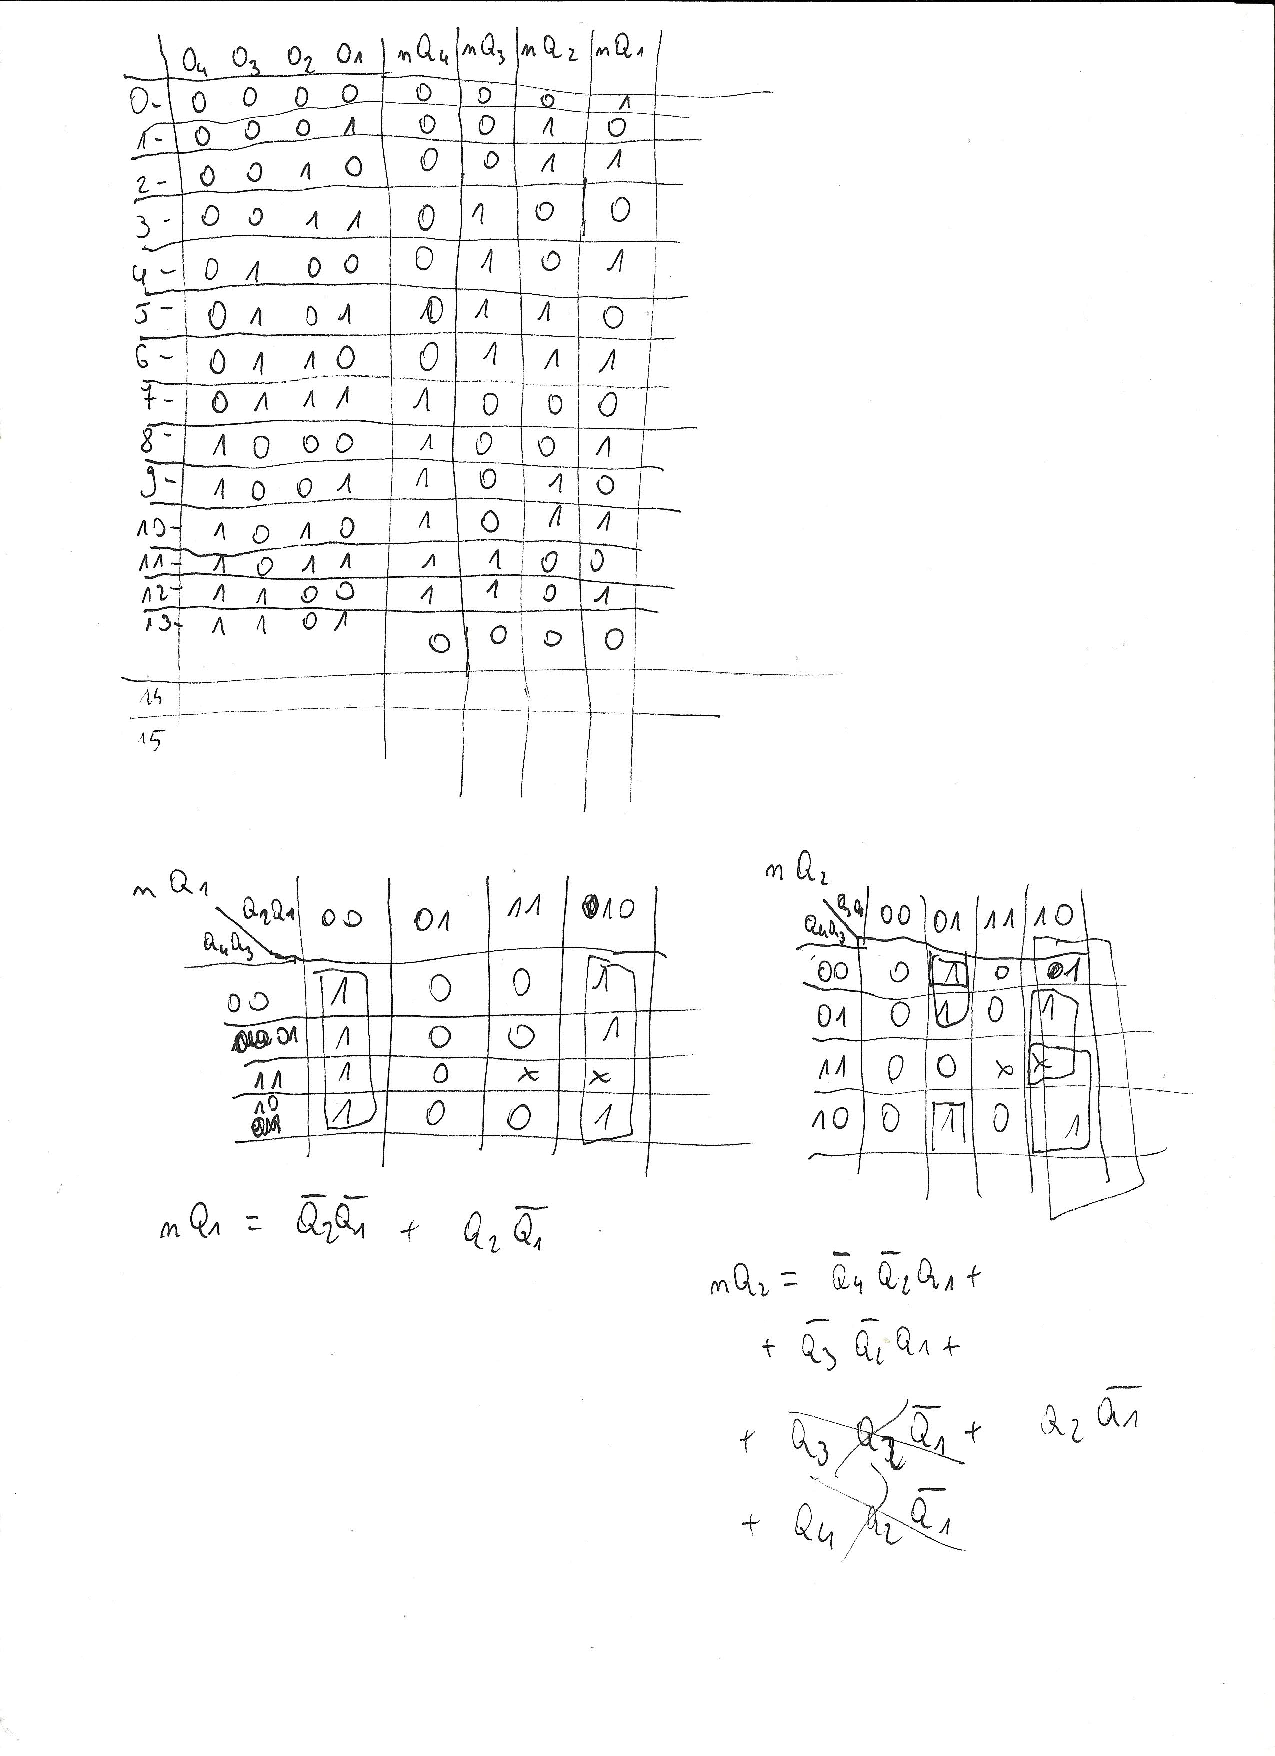
\includepdf{1}

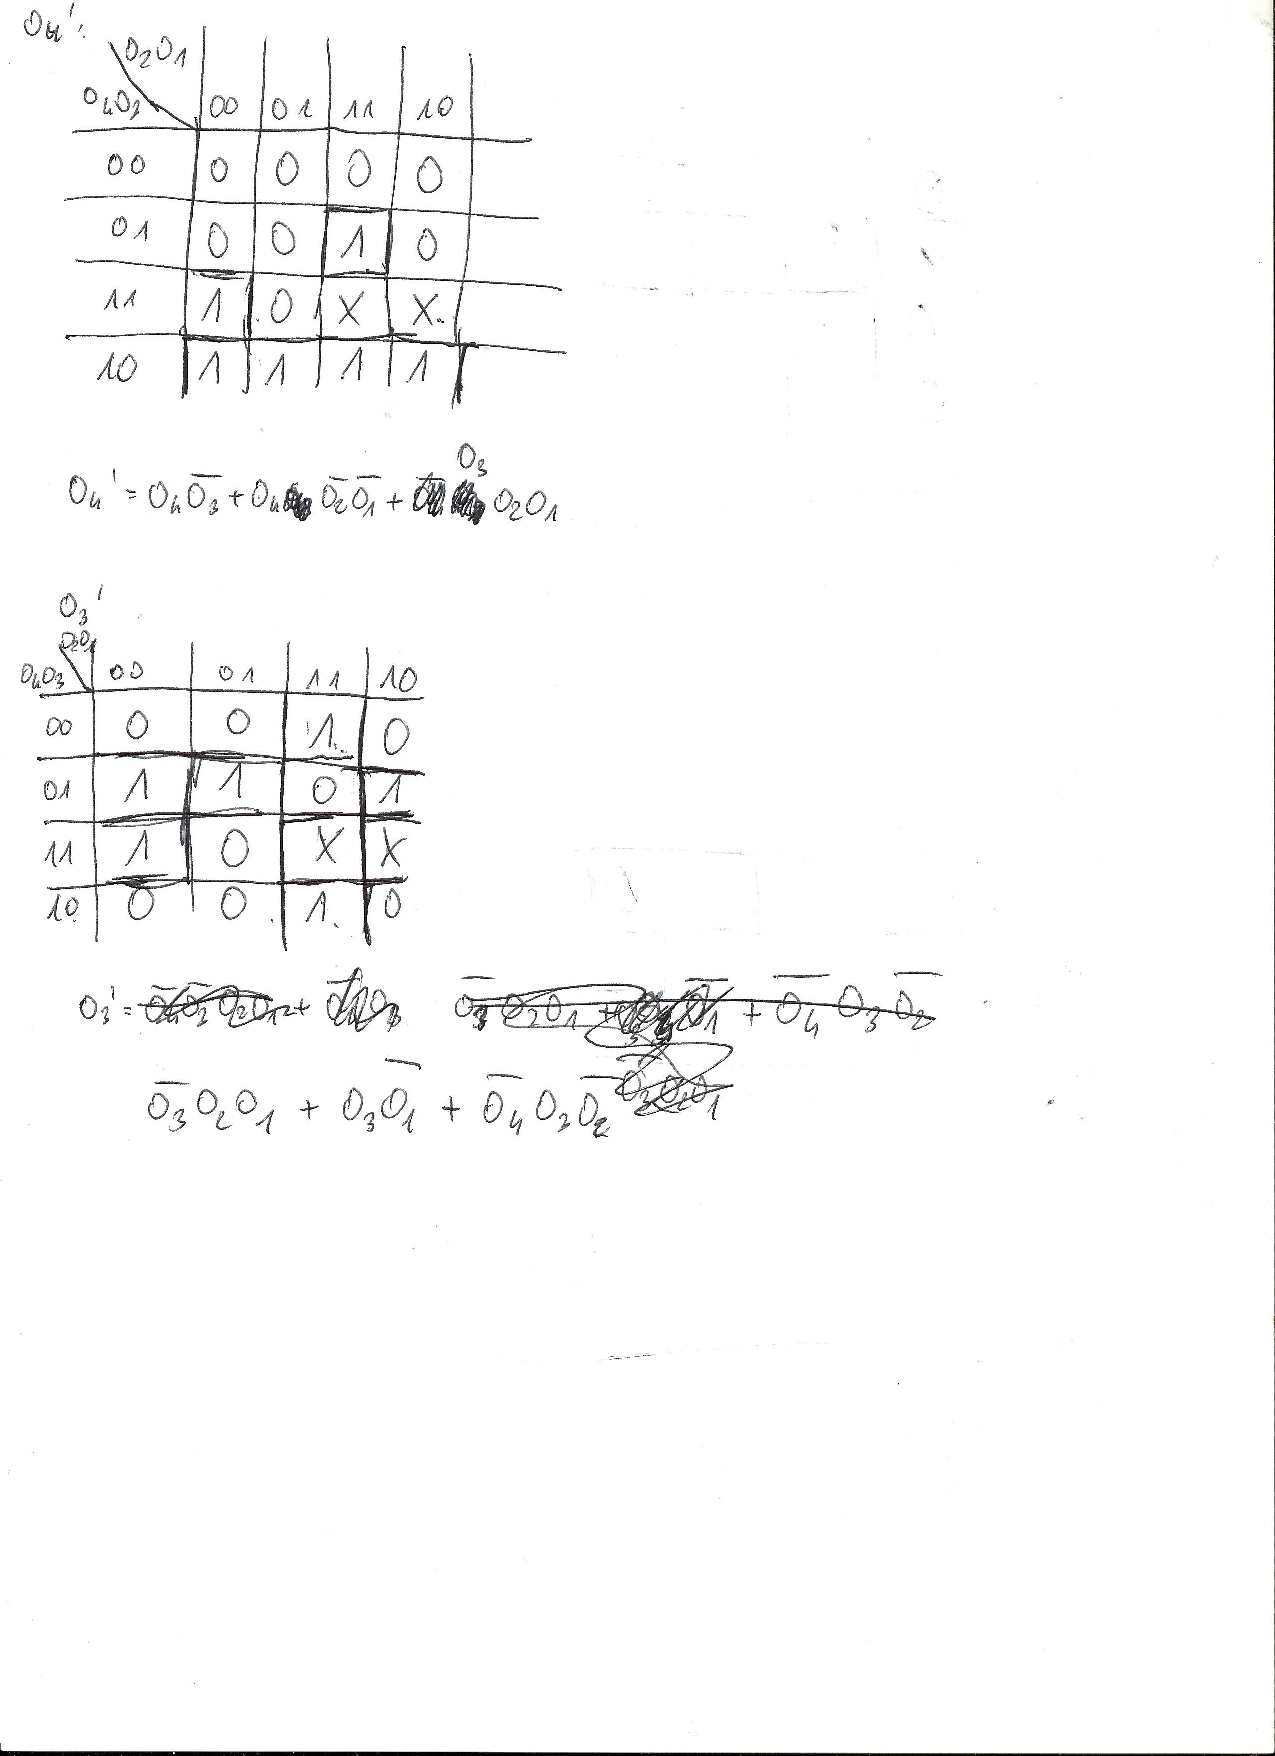
\includepdf{2}

\newpage

Natomiast na poniższej tabeli zaprezentowana jest zworkowa realizacja licznika.

\begin{figure}[h!]
\centering
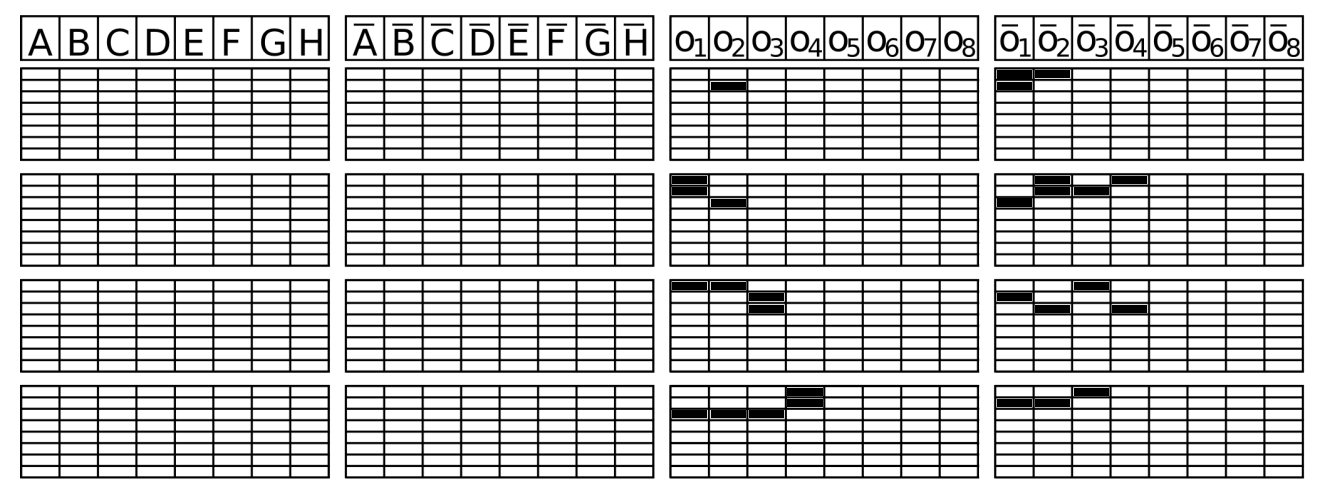
\includegraphics[width=18cm, height=9cm]{licznik_modulo}
\end{figure}

\subsection{3 bitowy licznik sterowany sygnałem A w kodzie Grey'a}
\label{3bit}

Kolejnym poleceniem było wykonanie 3 bitowego licznika w kodzie Grey'a (punkt \ref{grey}), który w zależności od sygnału A wykonywał poniższe funkcje:
\begin{itemize}
\item A = 0 => Licznik zmienia się od 1 -> 6 w górę
\item A = 1 => Rotate right - przesunięcie bitowe w prawo. (punkt \ref{przesbit})
\end{itemize}

Poniżej znajdują się zeskanowane tabele Karnaugh'a, które przedstawiają trzy konieczne funkcję, które składają się na ten układ.

\newpage

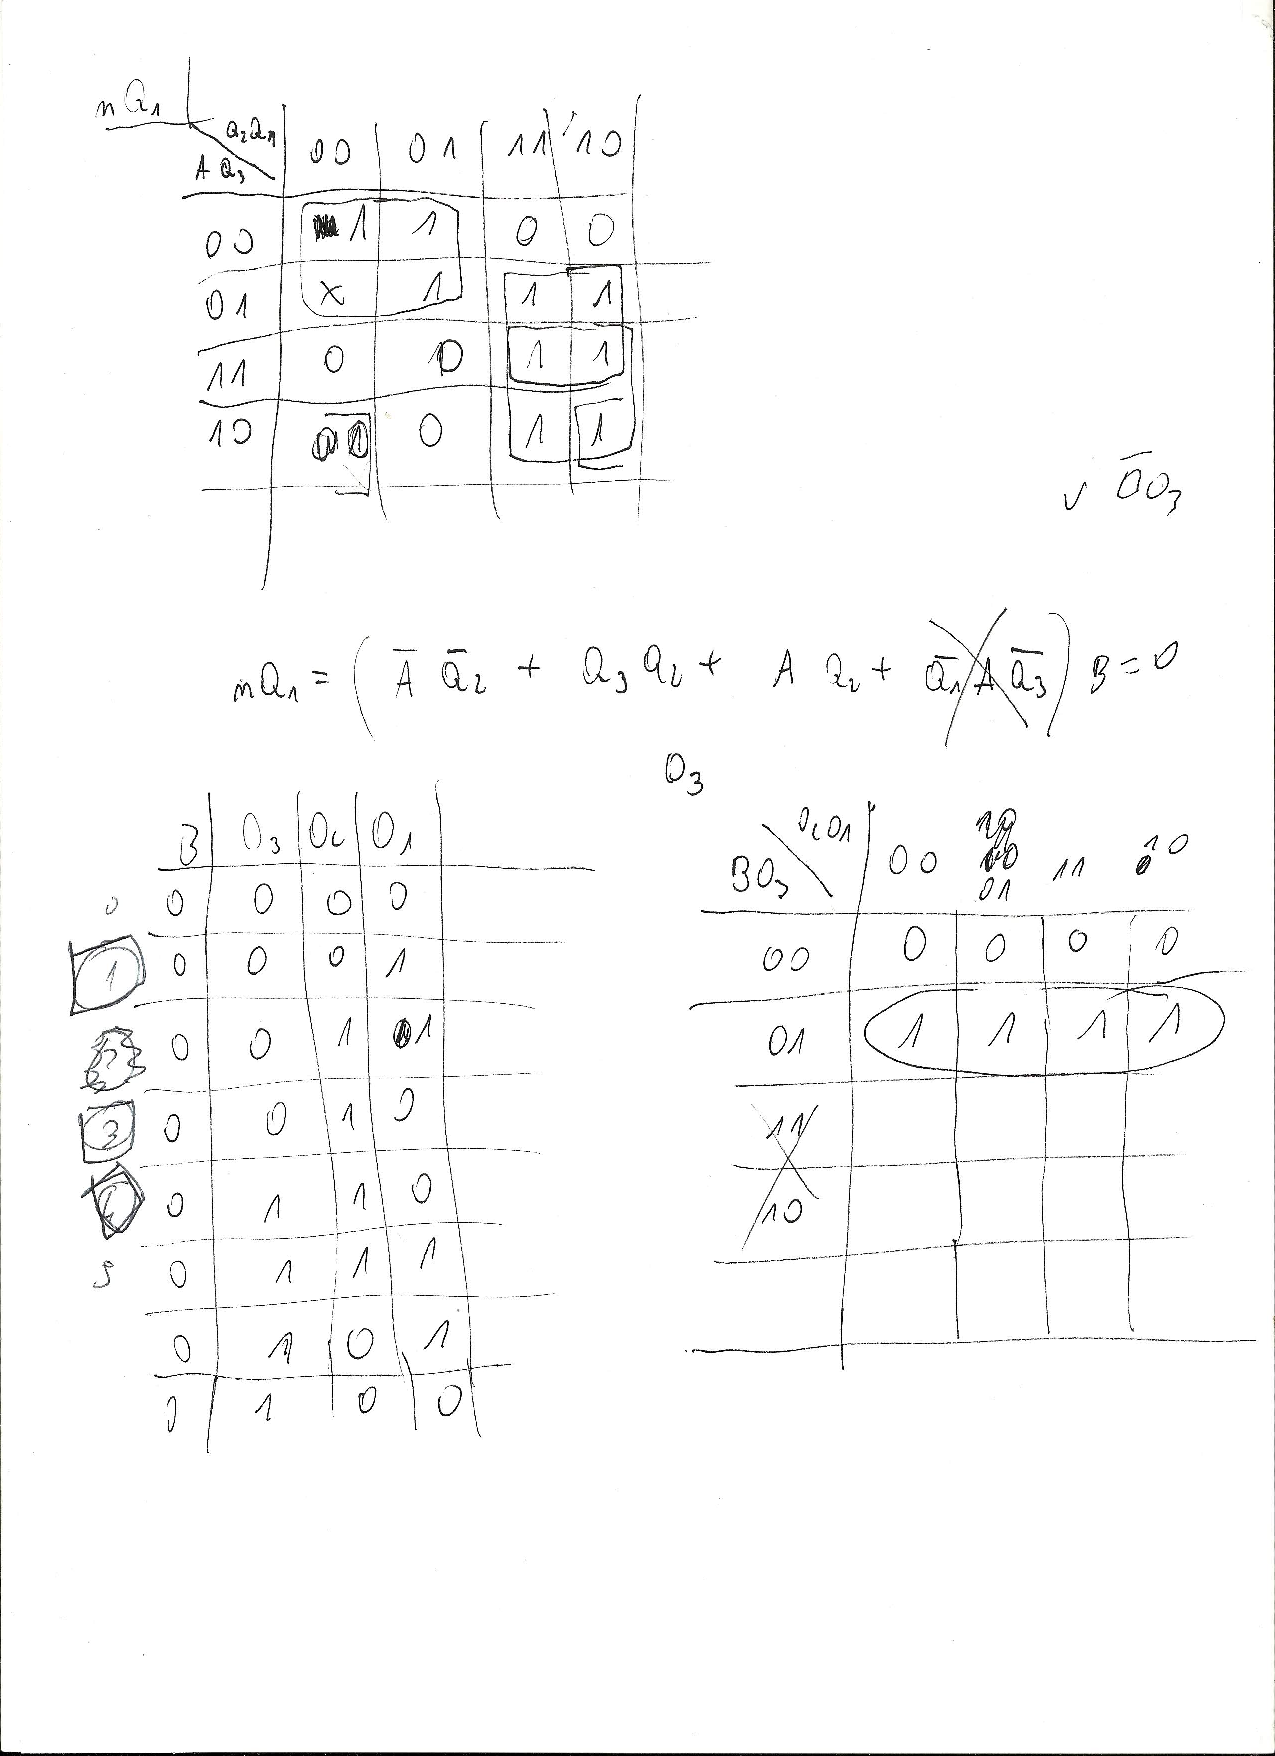
\includepdf{3}

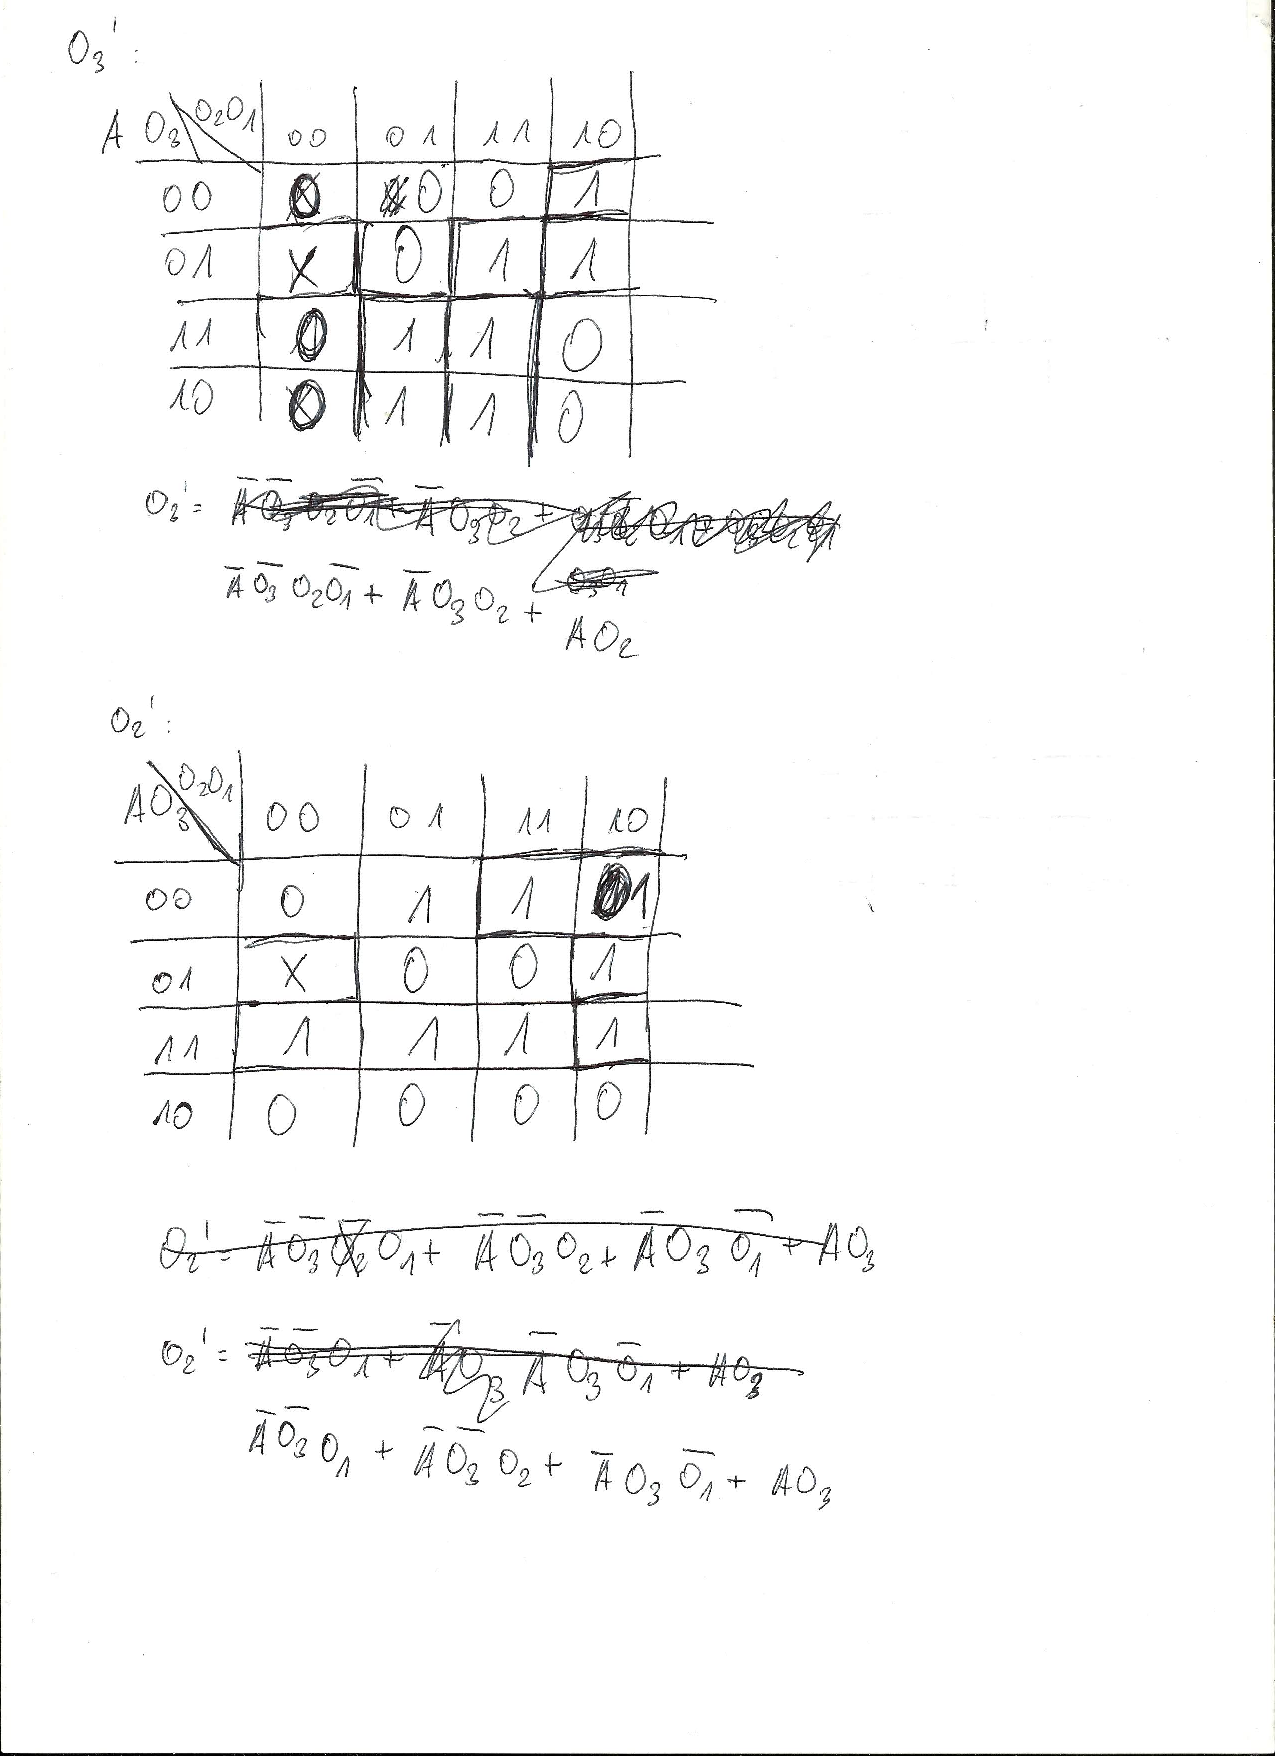
\includepdf{4}

\newpage

Natomiast poniżej można zaobserwować reprezentację zworkową tychże funkcji na matrycy PLD.

\begin{figure}[h!]
\centering
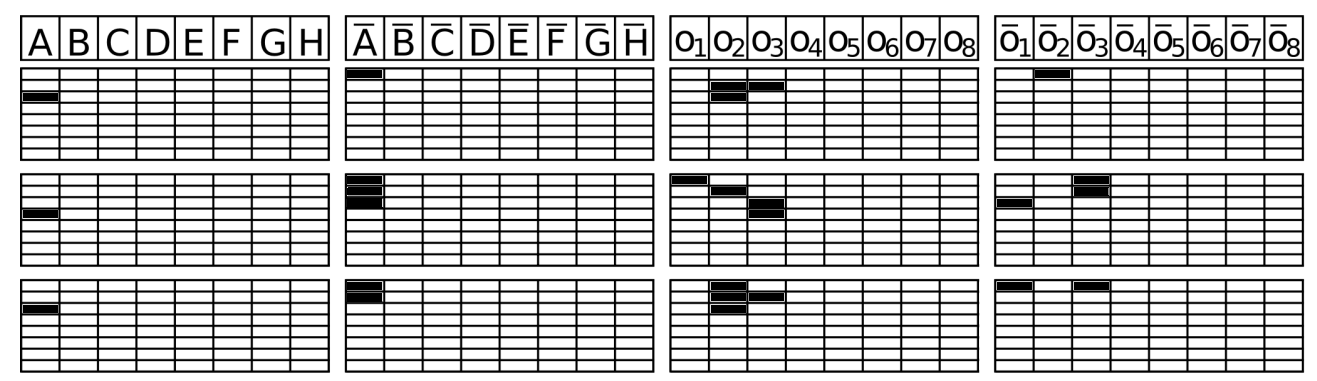
\includegraphics[width=18cm, height=7cm]{licznik_grey}
\end{figure}

\subsection{3 bitowy licznik sterowany sygnałem A w kodzie Grey'a, które zapamiętuje stan}

Ostatnim poleceniem było przerobienie w taki sposób licznika z punktu \ref{3bit}, aby licznik w momencie, gdy sygnał B = 0 zatrzymywał się.
Okazało się, że jedynym krokiem, jaki musimy zrobić to dodać  B do aktualnych członów funkcji oraz dodać OR zanegowane B, aktualna funkcja.

Finalnie poniżej znajdują się zapisane funkcje: \\
$O_{1}' = B(\overline{AO_{2}} + O_{3}O_{2} + AO_{2}) + \overline{B}O_{1}$ \\ \, \\
$O_{2}' = B(\overline{AO_{3}}O_{1} + \overline{AO_{3}}O_{2} + \overline{AO_{1}}O_{3} + AO_{3}) + \overline{B}O_{2}$ \\ \, \\
$O_{3}' = B(\overline{AO_{3}O_{1}}O_{2} + \overline{A}O_{3}O_{2} + AO_{2}) + \overline{B}O_{3}$ \\

Poniżej znajduje się reprezentacja zworkowa finalnego licznika:

\begin{figure}[h!]
\centering
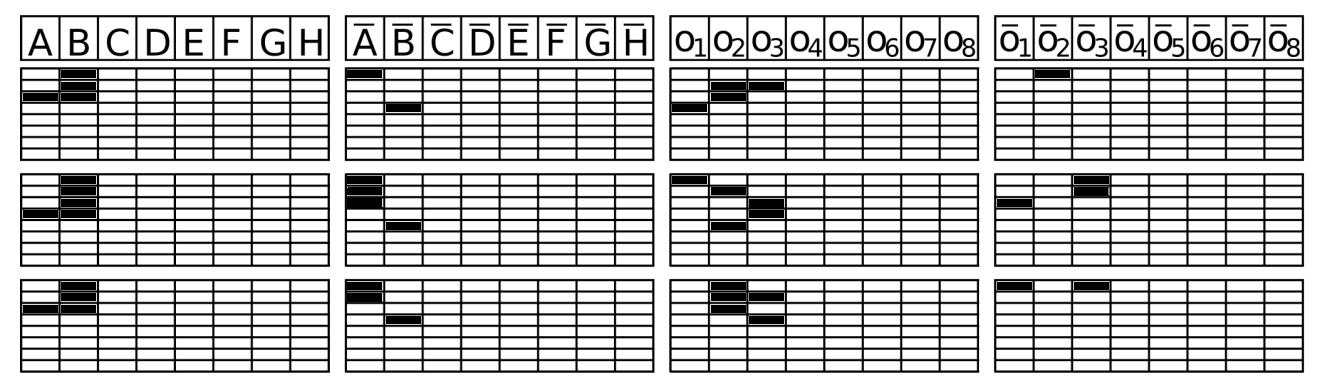
\includegraphics[width=18cm, height=7cm]{licznik_grey_B}
\end{figure}

\end{justify}
\end{document}